\section{Methods}
\label{sec:methods}


\subsection{Overview}
\label{subsec:methods:overview}

Here we provide a brief overview of the several methods described in this manuscript.
First, we rely on CLAM (Clustered Learning of Approximate Manifolds) as a fairly na\"ive clustering method; CLAM derives from CHESS~\cite{ishaq2019clustered} but introduces significant novelty: while CHESS only clustered to a pre-specified depth for the \emph{sole} purpose of search, CLAM uses a similar clustering on several training sets not included in testing to learn data properties for which anomaly detection will perform well across those datasets.
Unlike CHESS, CLAM does not use a specific depth to halt clustering; instead, it tracks properties including local fractal dimension, cluster cardinality, and moving averages thereof, based upon a training dataset.
The motivation behind these properties is driven by the manifold hypothesis: as the divisive clustering begins to ``separate'' different regions of the manifold, the fractal dimension and cluster cardinality should begin to change; ideally, we seek clusters that optimally ``cover'' the manifold as described in~\cite{yu2015entropy}, though these clusters will clearly not all be at the same depth of the tree across the manifold.
Clustering too deeply will lead to locally uniform-density clusters of \emph{high} fractal dimension, while clustering too shallowly will lead to clusters that contain highly varied regions of the manifold.
We seek to find the optimal balance such that the clusters discover the structure of the manifold.
The stopping criteria are described in Section~\ref{subsubsec:methods:clam:clustering}.
Importantly and novelly, these stopping criteria are not uniform for a given dataset; they are adaptive with differing properties of different regions of the manifold, and may exist at different depths of the tree (see Figure~\ref{fig:methods:graph-generation}).
Also novelly, a graph is induced from the overlap among clusters at this set of depths (see Section~\ref{subsec:methods:induced-graphs}, and this graph informs the CHAODA anomaly-detection algorithms that CLAM enables (see Section~\ref{subsec:methods:individual-algorithms}).
CHAODA relies on an ensemble-learning approach based on six simple heuristics; the ensemble-learning approach is described in Section~\ref{subsec:methods:ensemble}.
These distinct heuristics attempt to encompass distinct notions of what make a datapoint anomalous: is it truly isolated, or is the distribution of datapoints multi-modal, or is it very low-dimensional despite being embedded in a high-dimensional space?

In all, CLAM builds on a clustering algorithm originally developed for a different purpose (accelerated approximate search) and uses a novel graph-inference approach to enable several anomaly-detection heuristics that are effective in practice.

\begin{figure*}[ht!]
    \centering
    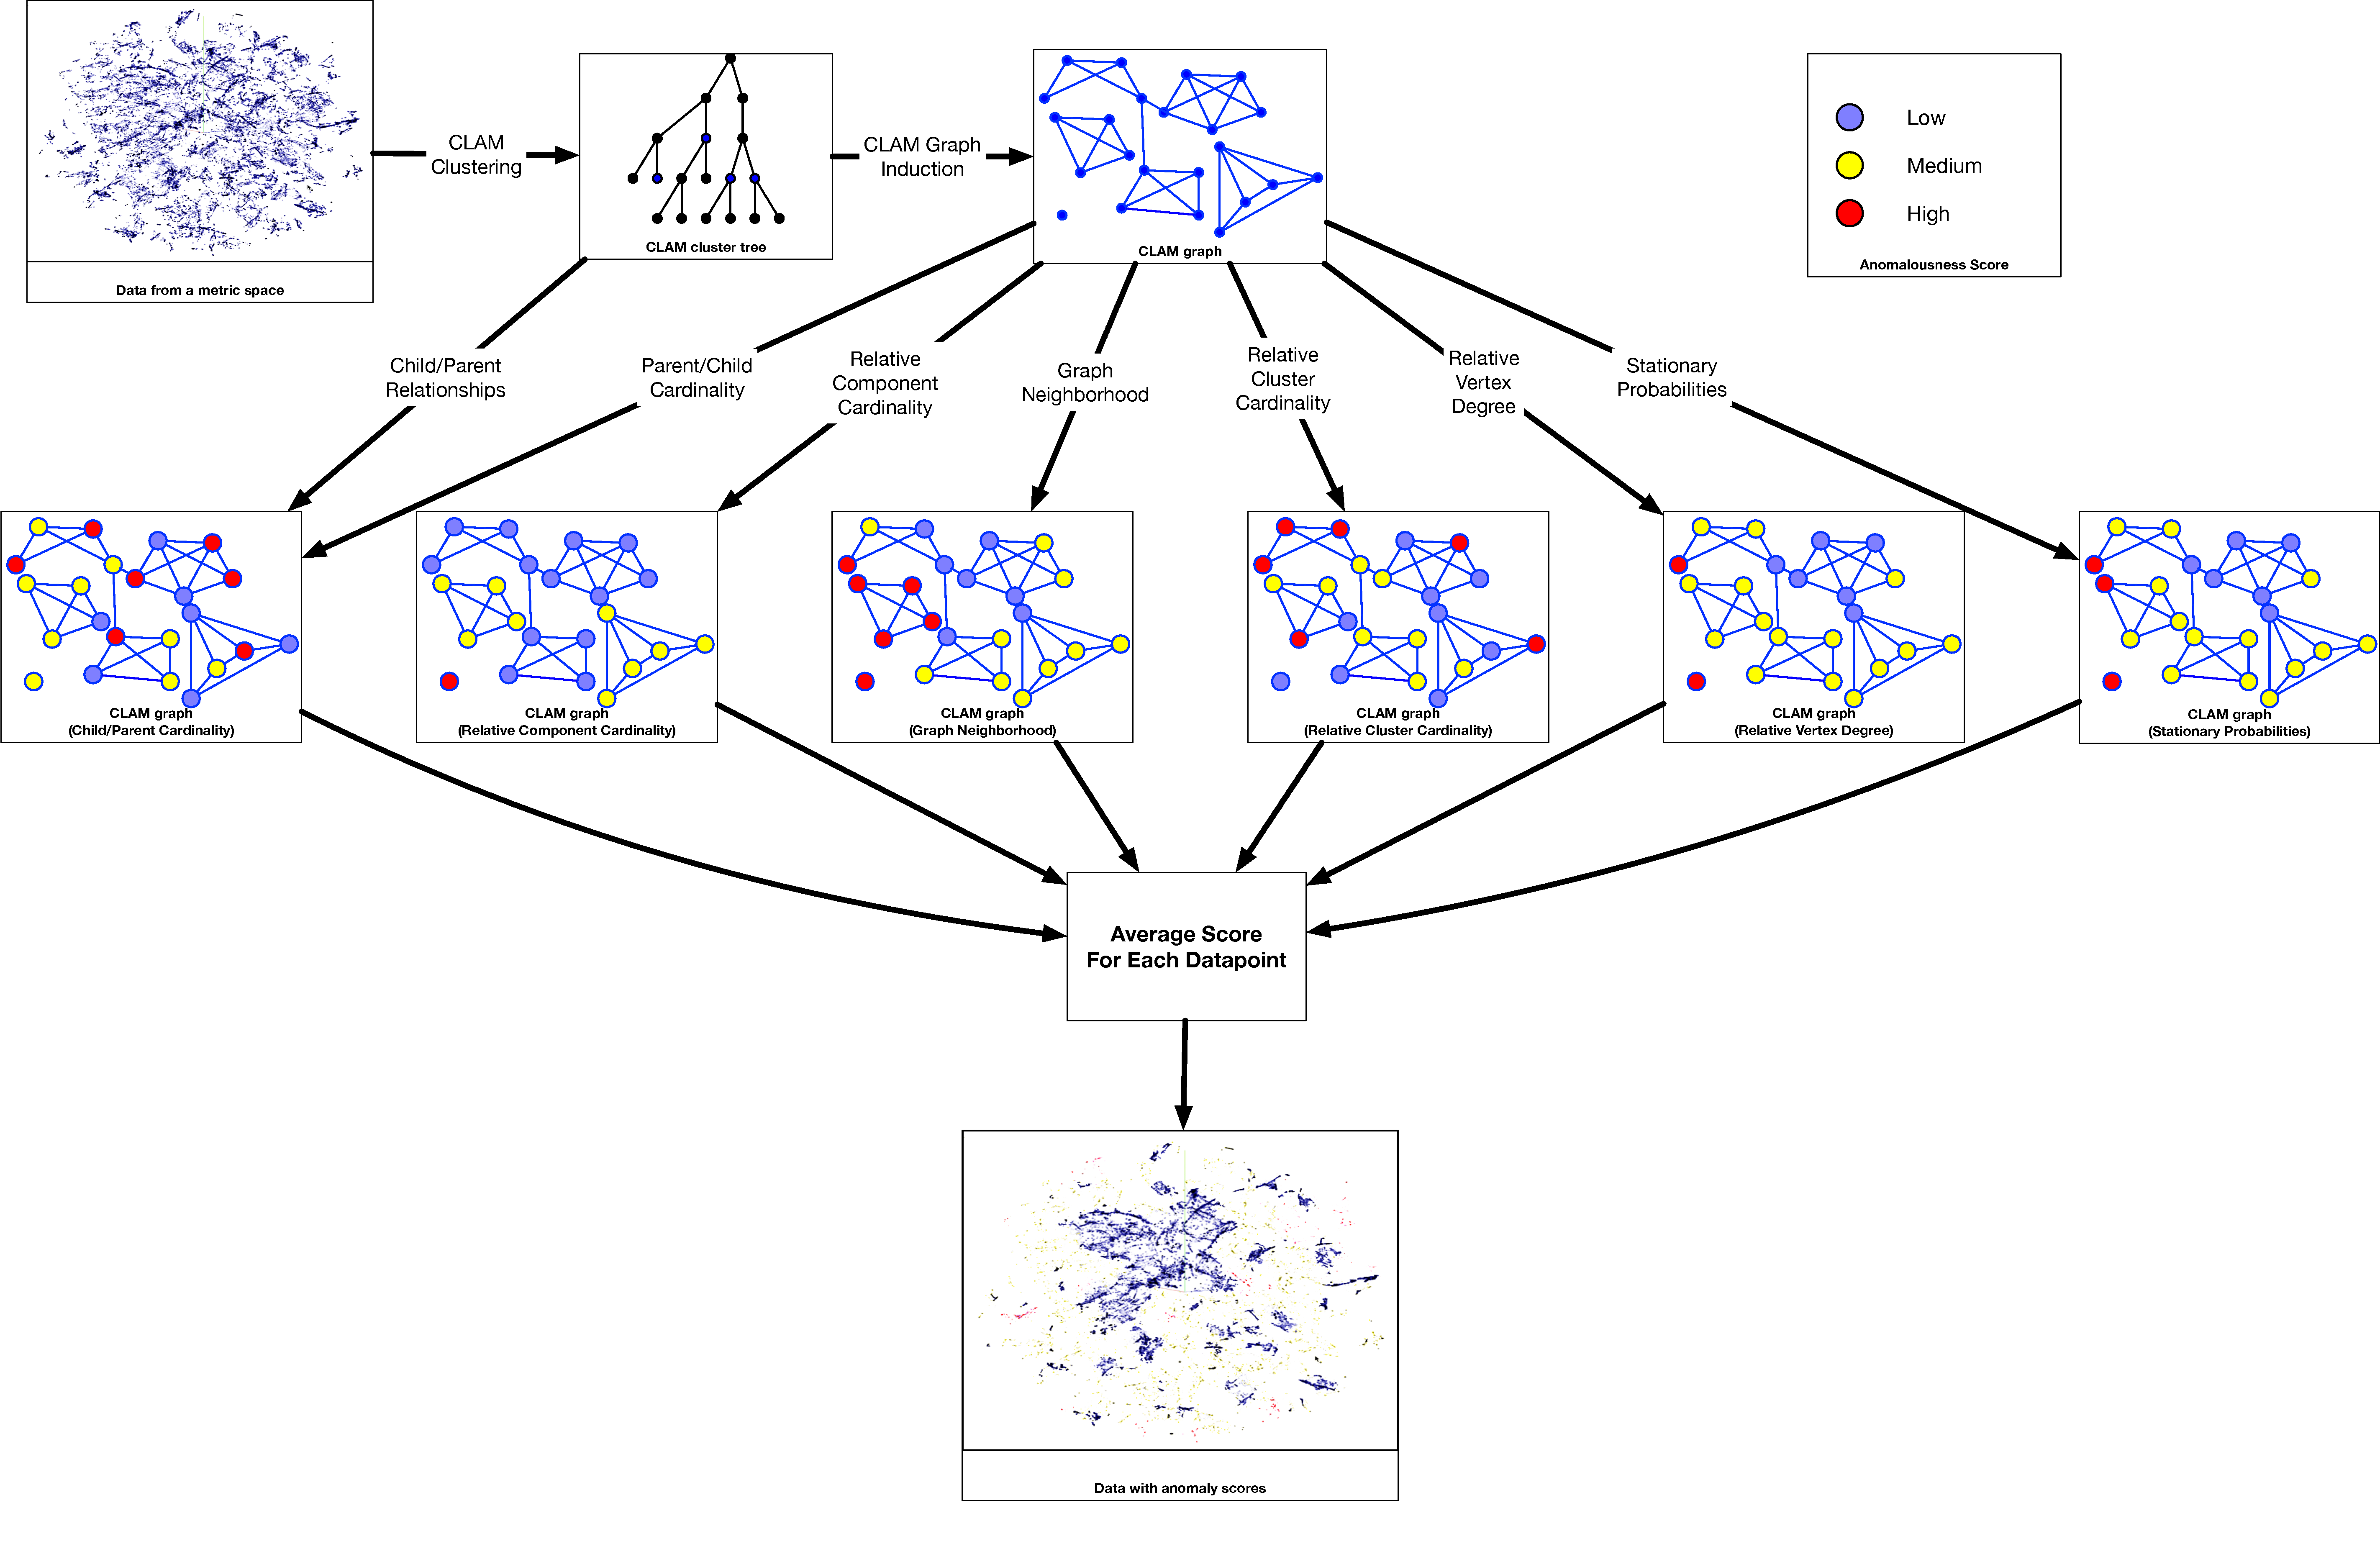
\includegraphics[width=6in]{images/chaoda-workflow.pdf}
    \caption{Overview of the CHAODA workflow.
        Blah blah. Say something about arbitrary color scheme, and note e.g. similarity between degree and stationary distribution. Walk through flow.}
    \label{fig:methods:chaoda-workflow}
\end{figure*}


\subsection{CLAM}
\label{subsec:methods:clam}

We present a manifold-mapping algorithm called CLAM (Clustered Learning of Approximate Manifolds).
CLAM requires a dataset and a distance function.
A dataset is a collection of $n$-points embedded in a $D$-dimensional Banach space, $\textbf{X} = \{x_1 \dots x_n\}, x_i \in \mathbb{R}^D$.
A Distance Function takes two points in the dataset and deterministically produces a non-negative real number, $f : (\mathbb{R}^D, \mathbb{R}^D) \mapsto \mathbb{R}^+$.
The distance must be such that $f(x, x) = 0$ and $f(x, y) = f(y, x)$ $\forall x, y \in X$.
The distance function may or may not obey the triangle inequality.
In this paper we used $L1$-norm and $L2$-norm, which are metrics;
however, CLAM and CHAODA are general over any distance function that obeys these properties.
We provide proofs of the complexity of each algorithm in the Supplement.


\subsubsection{Clustering}
\label{subsubsec:methods:clam:clustering}

We start by building a divisive hierarchical clustering of the data based on a pair of well-separated points from a random sampling of $\sqrt k$ points from the $k$ points in a given cluster from the tree.
This achieves clustering in expected $\mathcal{O}(n \lg n)$ time.
CLAM clustering is defined in Algorithm~\ref{alg:clam-partition}.
The procedure is inspired from~\cite{ishaq2019clustered}, although we have improved upon their partition method.
The root cluster contains all points and clusters are recursively partitioned until each leaf cluster contains only one point.
% We can't cite our work as "us" during the review process

\begin{algorithm} % enter the algorithm environment
\caption{Partition} % give the algorithm a caption
\label{alg:clam-partition} % and a label for \ref{} commands later in the document
\begin{algorithmic}[1] % enter the algorithmic environment
    \REQUIRE $cluster$
    \STATE $k \leftarrow \lfloor \sqrt{|cluster.points|} \rfloor$
    \STATE $seeds \leftarrow k$ random points from $cluster.points$
    \STATE $c \leftarrow$ geometric median of $cluster.points$
    \STATE $r \leftarrow \argmax d(c,x) \ \forall \ x \in cluster.points$
    \STATE $l \leftarrow \argmax d(r,x) \ \forall \ x \in cluster.points$
    \STATE $cluster.left \leftarrow \{x | x \in cluster.points \land d(l,x) \le d(r,x)\}$
    \STATE $cluster.right \leftarrow \{x | x \in cluster.points \land d(r,x) < d(l,x)\}$
    \IF{$|cluster.left| > 1$}
        \STATE Partition(cluster.left)
    \ENDIF
    \IF{$|cluster.right| > 1$}
        \STATE Partition(cluster.right)
    \ENDIF
\end{algorithmic}
\end{algorithm}

These clusters have several interesting and important properties for us to consider.
These include the \textit{cardinality}, the number of points in a cluster;
\textit{center}, the geometric median of points contained in a cluster;
\textit{radius}, the distance to the farthest point from the center;
and \textit{local fractal dimension},
as given by:

\begin{gather}
    \log_2\bigg(\frac{|B_D(c, r)|}{|B_D(c, \frac{r}{2})|}\bigg)
    \label{fractal-dimension}
\end{gather}

where $B_D(c,r)$ is the set of points contained in a ball on the dataset $D$ of radius $r$ centered on a point $c$~\cite{ishaq2019clustered}.
Thus, this measure captures the ``spread'' of datapoints on the manifold in comparison to the (typically much larger) embedding space, motivated by the notion that CLAM's learned graph will adapt its ``resolution'' to different regions of the manifold.

We can also consider individual \textit{parent-child ratios} of cardinality, radius, and local fractal dimension, as well as the \textit{exponential moving averages} of those parent-child ratios along a branch of the tree.
In particular, we use the parent-child ratios and the exponential moving averages of those ratios to generalize our method from a small set of training datasets to a large, distinct set of testing datasets.


\subsubsection{Graphs}
\label{subsubsec:methods:clam:graphs}

Clusters that are close in the embedding space sometimes have overlapping volumes; i.e.,\ the distance between their centers is less than or equal to the sum of their radii.
We define a graph $G=(V,E)$ with the selected clusters in one-to-one correspondence to vertices and with an edge between two vertices if and only if their clusters overlap.
While it is fairly standard in the literature to define graphs using this geometric property of overlapping volumes, the challenge is in selecting the right clusters to build useful graphs.
This selection process, presented in Section~\ref{subsec:methods:induced-graphs}, is among the major novel contributions of CLAM and CHAODA.

Figure~\ref{fig:methods:graph-generation} illustrates how CLAM induces a graph from non-uniform depths in a cluster tree.
Interestingly, the clusters are not necessarily hyperspheres, but polytopes akin to a high-dimensional Voronoi diagram~\cite{voronoi1908nouvelles}.

For our purposes, a graph exhibits an important invariant.
The clusters corresponding to vertices in the graph collectively contain every point in the dataset.
In addition, each point in the dataset is in exactly one cluster in the graph.
A corollary to this invariant is that a graph will never contain two vertices such that one vertex corresponds to an ancestor or descendant cluster of another vertex.
A graph can be built from clusters at a fixed depth in the cluster-tree (a layer-graph), or from clusters from multiple different depths in the tree (an optimal-graph).
This graph need not be fully connected, and in practice often contains many small, disjoint connected components.
In this work we consider the cardinality of a graph to be \textit{vertex cardinality}; i.e.,\ the number of vertices (clusters) in the graph.


\subsubsection{The Manifold}
\label{subsubsec:methods:clam:the-manifold}
According to the ``manifold hypothesis''~\cite{fefferman2016testing}, datasets collected from constrained generating processes that are embedded in a high-dimensional space typically only occupy a low-dimensional manifold in that space.
The graphs discussed thus far map this low-dimensional manifold in the original embedding space.
Different graphs do this at different levels of local or global resolution.
Our aim is to build a graph where different resolutions may be necessary for different regions of the manifold.
We can then apply several anomaly detection algorithms to these graphs.

We describe a set of algorithms in Section~\ref{subsec:methods:individual-algorithms}.
While mainly relying on graph information, these algorithms can also incorporate information from the tree, such as the child-parent cardinality ratio method described in Section~\ref{subsubsec:methods:individual-algorithms:cpcr}.
While these algorithms are themselves fairly simple, the real challenge is in selecting the right clusters for the graphs for these algorithms to operate upon.
We will demonstrate CLAM's manifold mapping and graph selection to be effective enough that even these simple algorithms, more often than not, outperform competing state-of-the-art algorithms.


\subsection{Induced Graphs}
\label{subsec:methods:induced-graphs}

The heart of the problem with CHAODA is building the right graph(s) to represent the underlying manifold.
One could try using every possible combination of clusters to form every possible graph but this leads to combinatorial explosion.
Instead, we must intelligently select those clusters that build a graph which will perform well for anomaly detection.

Area under the curve (AUC) of the receiver operating characteristic (ROC) is often used to measure the performance of anomaly detectors;
we wish to choose clusters that are expected to maximize this measure.
We use the definition of AUC-ROC based on CHAODA being an \emph{unsupervised} model where ground truth can be examined post-hoc from the datasets; a score is given to every point, and the AUC is computed in the usual fashion~\cite{fawcett2006introduction}.
The ground-truth labels are only used during training for the training set of datasets, while the ground-truth for the test set of datasets is used purely for post-hoc performance calculations.
Thus, CHAODA is supervised only in the sense of learning where to build a graph on training datasets, but unsupervised on any new (e.g. test) datasets.

We find the ``right graphs'' by learning a function that takes the parent-child ratios of cardinality, radius and local fractal dimension and the exponential moving averages (from the root to the cluster) of these ratios for a cluster and predicts the contribution to AUC-ROC of selecting that cluster for the graph.
We thus need to learn a function of the form $f: \mathbb{R}^6 \mapsto \mathbb{R}^+$ that takes these six ratios learn the AUC from the scores assigned to points in the corresponding cluster.
By using these parent-child ratios and exponential moving averages thereof, we gain some agnosticity to dataset-specific properties and instead learn geometric and topological properties that generalize over datasets in Banach Spaces that obey the Manifold Hypothesis.
This is essentially transfer learning: we will learn such functions from a set of datasets \emph{completely distinct from} the set of datasets we use for benchmarking.
We are effectively learning a set of criteria that can enable selection of a useful depth (perhaps not truly optimal), varying along the cluster tree, with regards to anomaly detection.

We choose a linear regression model and a regression tree model to fill this role.
Such models require training data.
To generate this data, we take a random sample from the datasets described in Section~\ref{subsec:methods:datasets}, choosing six datasets at random with between 1,000 and 100,000 points.
We generate a clustering for each dataset, and start by inducing several uniform-depth (layer) graphs from the tree.
We apply each individual algorithm described in Section~\ref{subsec:methods:individual-algorithms} to each such graph and, using the labels, we calculate the AUC over the subset of points in each cluster.
We use that AUC as the training target for our meta-ml models.
The corresponding feature vector is, as stated earlier, the six-element vector of the parent-child ratios and their exponential moving averages.
This concludes the first epoch of training and gives us a set of trained meta-ml models.
For each subsequent epoch of training, we use the meta-ml models from the previous epoch to rank the clusters in each tree (corresponding to each training dataset) and select graphs that perform better, as measured by AUC-ROC, for anomaly detection.
Each epoch, thus, iteratively improves the meta-ml models used to select graphs and each newly selected graph produces better data for the meta-ml models to be used in the next epoch.

Once we are satisfied with the performance of our meta-ml models on the set of training datasets, we freeze the meta-ml models and use them to select graphs for the test set of datasets.
Since the ratios used to train and predict from these meta-ml models are agnostic to dataset specific properties such as cardinality and dimensionality, the trained models transfer from the training set of datasets to the \textit{completely distinct} test set of datasets.

\begin{figure}[ht!]
    \centering
    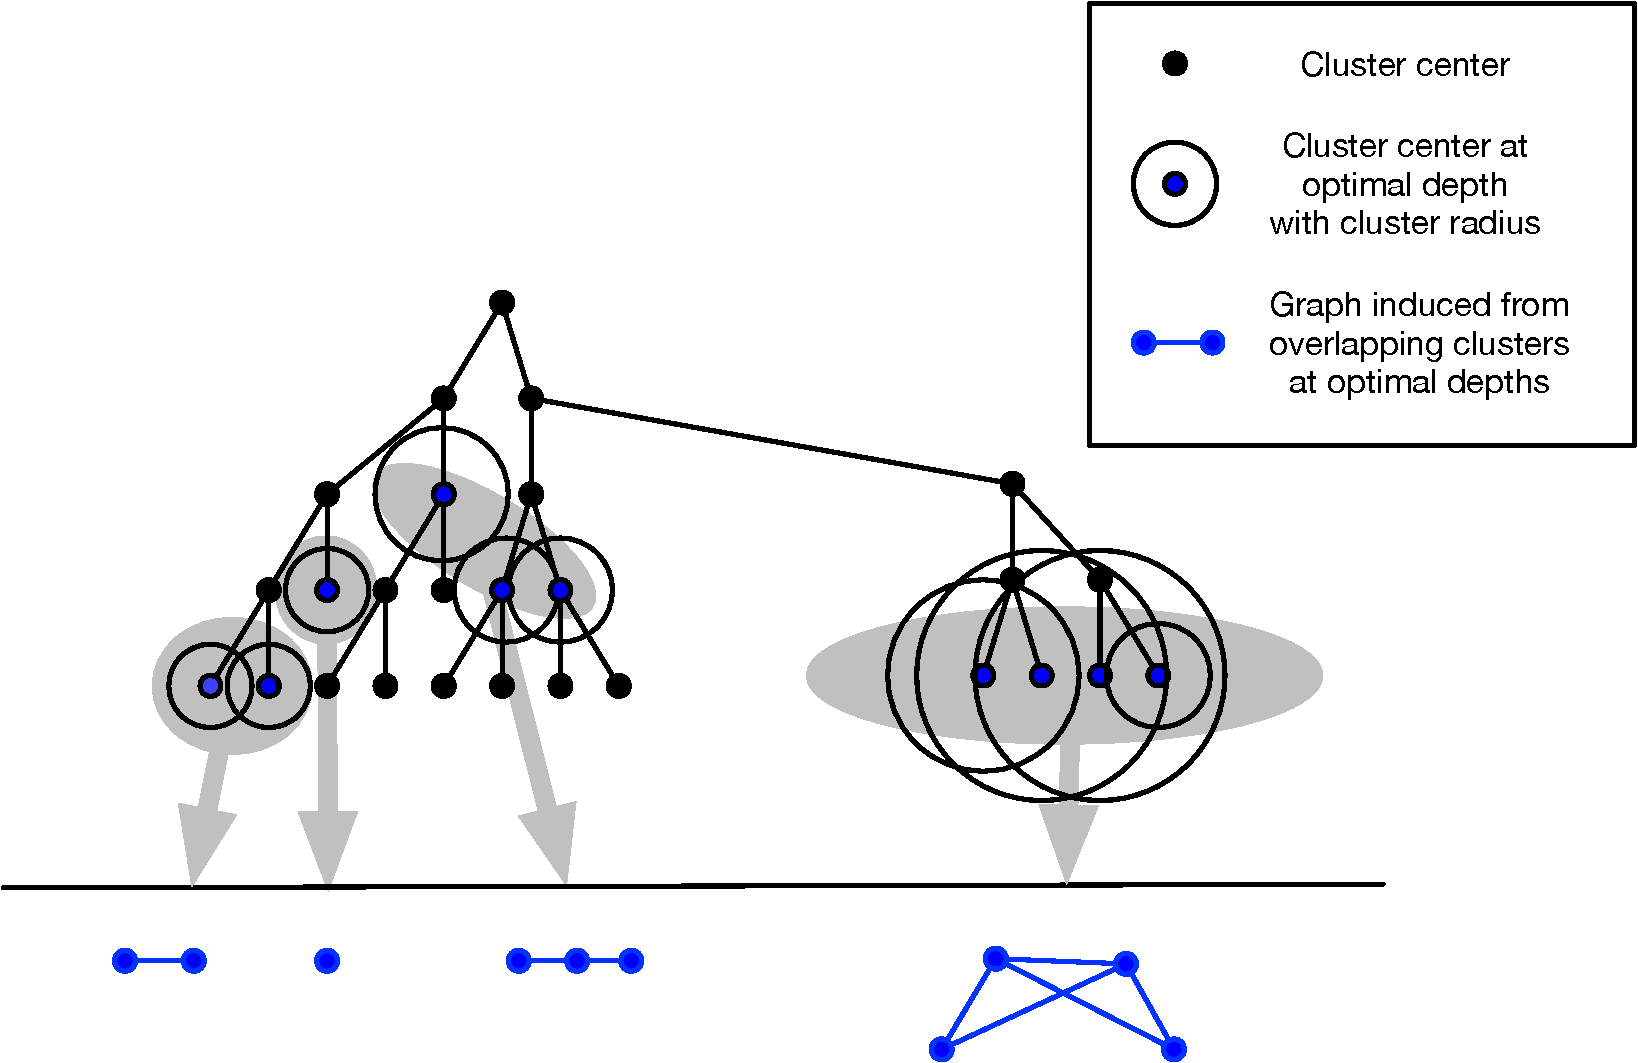
\includegraphics[width=2.5in]{images/tree-graph.pdf}
    \caption{Using CLAM to induce a graph from a cluster tree.
        Dots in the tree represent cluster centers;
        blue dots represent centers of chosen clusters.
        Circles represent the volume of a cluster (the radius is the distance from the center to the furthest point contained within that cluster).
        Gray arrows point to the induced graph components, which are indicated in blue below the horizontal line.}
    \label{fig:methods:graph-generation}
\end{figure}


\subsection{Individual Algorithms}
\label{subsec:methods:individual-algorithms}

The key to an effective ensemble method is that each component algorithm contributes a unique inductive bias~\cite{chen2017outlier}.
Here we describe six simple algorithms for anomaly detection, each using a CLAM graph to calculate an anomalousness score for each datapoint.
For each algorithm, we note the intuition behind its contribution to the ensemble.
In the following, $scores$ is a dictionary of clusters and their outlier scores,
$V$ and $E$ are the sets of clusters and edges in a graph, respectively, and $|c|$ is
the cardinality of a cluster $c$, the number of points in that cluster.


\subsubsection{Relative Cluster Cardinality}
We measure the anomalousness of a point by the cardinality of the cluster that the point belongs to relative to the cardinalities of the other clusters.
Points in the same cluster are considered equally anomalous and points in clusters with lower cardinalities are considered more anomalous than points in clusters with higher cardinalities.
The algorithm is defined in Algorithm~\ref{alg:rclc}.
The time complexity is $\mathcal{O}(|V|)$.

\begin{algorithm}[h]
    \caption{Relative Cluster Cardinality}
    \label{alg:rclc}
\begin{algorithmic}[1]
    \REQUIRE $G$, a graph
    \FOR {cluster $c \in G$}
    \STATE $scores[c] \gets -|c|$
    \ENDFOR
\end{algorithmic}
\end{algorithm}


\subsubsection{Relative Component Cardinality}
We use the usual definition of connected components:
no two nodes from different components have an edge between them, and
every pair of nodes in the same component has a path connecting them.
Consider the relative cardinalities of each component in much the same way as we considered the relative cardinalities of clusters in the relative cluster cardinality method.
Points in clusters (vertices) in smaller components are considered more anomalous than those in larger components,
and points in clusters in the same component are considered equally anomalous.
The intuition here, as distinct from the previous algorithm, is to capture larger-scale structural information based on disjoint connected components from the CLAM graph.
The algorithm is defined in Algorithm~\ref{alg:rcc}.
This algorithm first finds the components of the graph, so its time complexity is $\mathcal{O}(|E| + |V|)$.

\begin{algorithm}[h]
    \caption{Relative Component Cardinality}
    \label{alg:rcc}
\begin{algorithmic}[1]
    \REQUIRE $G$, a graph
    \FOR {component $C \in G$}
        \STATE $scores[C] \gets -|C|$
    \ENDFOR
\end{algorithmic}
\end{algorithm}


\subsubsection{Graph Neighborhood}
Given the graph with clusters and edges, we consider the number of clusters reachable from a starting cluster within a given graph distance $k$.
We call this number the \textit{graph-neighborhood} of the starting cluster.
With $k$ small compared to the diameter of the graph, we consider the relative sizes of graph-neighborhoods of the clusters.
Points in clusters with small graph-neighborhoods are considered more anomalous than points in clusters with large graph-neighborhoods.
The intuition here is to capture information about the connectivity of the graph in the region around each cluster.
The algorithm is defined in Algorithm~\ref{alg:gns}.
This algorithm is dominated by computing the eccentricity of each cluster, so its time complexity is $\mathcal{O}(|E| \cdot |V|)$.

\begin{algorithm}[h]
    \caption{Graph Neighborhood}
    \label{alg:gns}
\begin{algorithmic}[1]
    \REQUIRE $G$, a graph
    \REQUIRE $f \in \mathbb{R}$ in the range $(0,1]$ ($0.25$ by default).
    \FOR {cluster $c \in G$}
        \STATE $e_c \gets$ the eccentricity of $c$
        \STATE $s \gets e_c \cdot f$
        \STATE perform a breadth-first traversal from $c$ with $s$ steps
        \STATE $v \gets$ the number of unique clusters visited by the traversal
        \STATE $scores[c] \gets -v$
    \ENDFOR
\end{algorithmic}
\end{algorithm}


\subsubsection{Child-Parent Cardinality Ratio}
\label{subsubsec:methods:individual-algorithms:cpcr}
As described in Section~\ref{subsubsec:methods:clam:clustering}, the partition algorithm used in clustering splits a cluster into two children.
If a child cluster contains only a small fraction of its parent's points (i.e., it only has a minority), then we consider the points in that child cluster to be more anomalous.
These child-parent cardinality ratios are accumulated for each point down its branch in the tree, terminating when the child cluster is a vertex in the induced graph.
Points with a low value of these accumulated ratios are considered more anomalous than points with a higher value.
This algorithm is inspired by iForest~\cite{tony2008iforest}, and captures information from the cluster tree directly, in addition to the CLAM graph.
The algorithm is defined in Algorithm~\ref{alg:cpcr}.
Unlike other CHAODA algorithms, this one accumulates parent scores into the children.
The time complexity of calculating the ratios is $\mathcal{O}(|V|)$ at clustering time, which is amortized over scoring the points;
the time complexity of scoring each individual point is $\mathcal{O}(1)$.

\begin{algorithm}[h]
    \caption{Child-Parent Cardinality Ratio}
    \label{alg:cpcr}
\begin{algorithmic}[1]
    \REQUIRE $G$, a graph
    \FOR {cluster $c \in G$}
        \STATE $p \gets$ the parent cluster of $c$
        \STATE $scores[c] \gets \frac{|p|}{|c|} + scores[p]$
    \ENDFOR
\end{algorithmic}
\end{algorithm}


\subsubsection{Stationary Probabilities}
\label{subsubsec:methods:individual-algorithms:sp}
We take an induced graph and assign each edge a weight inversely proportional to the distance between the centers of the two clusters that form that edge.
We compute the transition probability matrix of each component of the graph that contains at least two clusters.
These probabilities are stochastic over the edge weights for each cluster.
We then compute successive squares of this matrix.
This process will eventually converge as long as the graph is connected and aperiodic~\cite{levin2017markov}; we find this convergent matrix.
Consider the sum of the values along a row in the convergent matrix.
This is the expected proportion of visits to that cluster during a long random walk over the graph component.
We can consider this sum to be inversely related to the anomalousness of the corresponding cluster.
The intuition here is that less-reachable clusters are more likely to represent anomalous points.
The algorithm is defined in Algorithm~\ref{alg:sp}.
Its worst-case time complexity is $\mathcal{O}(|V|^{2.3728596})$ given by the matrix multiplication algorithm from~\cite{alman2021refined}.
In practice, however, this algorithm performs much better because the induced graphs are often composed of several small components rather than one large component.

\begin{algorithm}[h]
    \caption{Stationary Probabilities}
    \label{alg:sp}
\begin{algorithmic}[1]
    \REQUIRE $G$, a graph
    \FOR {component $C \in G$}
        \STATE $M \gets$ the transition matrix for $C$
        \REPEAT
            \STATE $M \gets M^2$
        \UNTIL $M$ converges
        \FOR {cluster $c \in C$}
            \STATE $s \gets $ the row from $M$ corresponding to $c$
            \STATE $scores[c] \gets -\Sigma(s)$ 
        \ENDFOR
    \ENDFOR
\end{algorithmic}
\end{algorithm}


\subsubsection{Relative Vertex Degree}
\label{subsubsec:methods:individual-algorithms:rvd}
For each cluster in the induced graph, consider the vertex degree, i.e. the number of edges connecting to that vertex, for each cluster in an induced graph.
We consider the points in a cluster with a high degree to be less anomalous than points in a cluster with low degree.
This is essentially a version of the previous algorithm that ignores edge weights, and may have different biases with regard to the sampling density of the dataset.
The time complexity is $\mathcal{O}(|V|)$.

\begin{algorithm}[h]
    \caption{Relative Vertex Degree}
    \label{alg:rvd}
\begin{algorithmic}[1]
    \REQUIRE $G$, a graph
    \FOR {cluster $c \in G$}
    \STATE $scores[c] \gets -cluster.degree$
    \ENDFOR
\end{algorithmic}
\end{algorithm}


\subsection{Ensemble}
\label{subsec:methods:ensemble}

Given a dataset and a list of distance functions for the dataset, we start by building a CLAM tree for each distance function on the dataset.
We extract the parent-child ratios and the exponential moving averages of those ratios for each cluster in each tree.
Given the set of meta-ml models learned from the training datasets as described in Section~\ref{subsec:methods:induced-graphs}, we use each model to rank every cluster.
The highest ranked clusters from each tree are then used to build a graph.
This gives us one graph for each combination of meta-ML model and distance function used.
We apply each of the six methods described in~\ref{subsec:methods:individual-algorithms} on each such graph.
With two meta-ML models (linear regression and regression trees) and two distance metrics ($L1$-norm and $L2$-norm), we have $24$ anomaly scores for each point in the dataset.
These scores are then combined into an ensemble by simply taking the mean of all scores for each point.
We present the AUC-ROC from this ensemble in Section~\ref{sec:results}.

% The individual algorithms described in~\ref{subsec:methods:individual-algorithms} produce outlier scores for each cluster, rather than for each point.
% We remedy this by assigning to each point the score of the cluster to which it belongs.
% Since our graphs guarantee that each point is in exactly one cluster and that every point from the dataset is accounted for, this assigns an outlier score to each point in a dataset.
Our individual methods produce scores with a wide range of values.
The only common feature among these scores is that low scores correspond to inliers and high scores correspond to outliers.
Therefore, we cannot directly compare scores across methods, which we need to be able to do for a functional ensemble.
Thus, we normalize the scores to the range $[0, 1]$, using gaussian normalization~\cite{kriegel2011interpreting}.
We include sigmoid and min-max normalization as options in our implementation.


\subsection{Datasets}
\label{subsec:methods:datasets}

We sourced 24 datasets containing only numerical features from Outlier Detection Datasets (ODDS)~\cite{rayana2016odds}.
All of these datasets were adapted from the UCI Machine Learning Repository (UCIMLR)~\cite{UCIMLR}, and were standardized by ODDS for benchmarks on anomaly and outlier detection.
Note that CHAODA is able to handle entirely-categorical datasets, but not mixed datasets.

We randomly select six datasets to train CHAODA: annthyroid, mnist, pendigits, satellite, shuttle, and thyroid.
We benchmarked CHAODA 30 times on the test datasets, with different random seeds.
We provide more details on the datasets in the Supplement.
During testing, we noticed that even though we often see $|V| \ll n $, the graph neighborhood size and stationary probabilities methods from~\ref{subsec:methods:individual-algorithms} were prohibitive, so we only run them when $|V| < max(128, \lfloor \sqrt n \rfloor)$.
We present these results in Table~\ref{table:results:test-performance} under the CHAODA-fast and CHAODA rows.
CHAODA-fast exhibits comparable performance to CHAODA, so we set CHAODA-fast as the default in our implementation.
All benchmarks were conducted on a 28-core Intel Xeon E5-2690 v4 2.60GHz, 512GB RAM and CentOS 7 Linux with kernel 3.10.0-1127.13.1.el7.x86\_64 \#1 SMP and Python 3.6.8.

CHAODA, being an unsupervised algorithm, is only compared against other unsupervised algorithms.
We compared against $18$ unsupervised algorithms collected in the pyOD suite~\cite{zhao2019pyod} and Scikit-Learn~\cite{pedregosa2011scikit}, as well as RS-Hash~\cite{sathe2016subspace}.
A supervised version of CHAODA is possible future work which will open up comparisons against supervised or weakly-supervised methods such as DAGMM~\cite{zong2018deep}.
